\section{Parsing and syntax trees}
\label{sect:parser_and_syntaxtrees}
Intro: basic parser prerequisites
The act of parsing is the process of analyzing a series of tokens and construct
a grammatical structure (syntax tree) based on a formally specified grammar. In
figure \ref{figure:parser:overview}, the parser component of a generic
compiler/interpreter is shown. 

\begin{figure}[h]
  \centering
    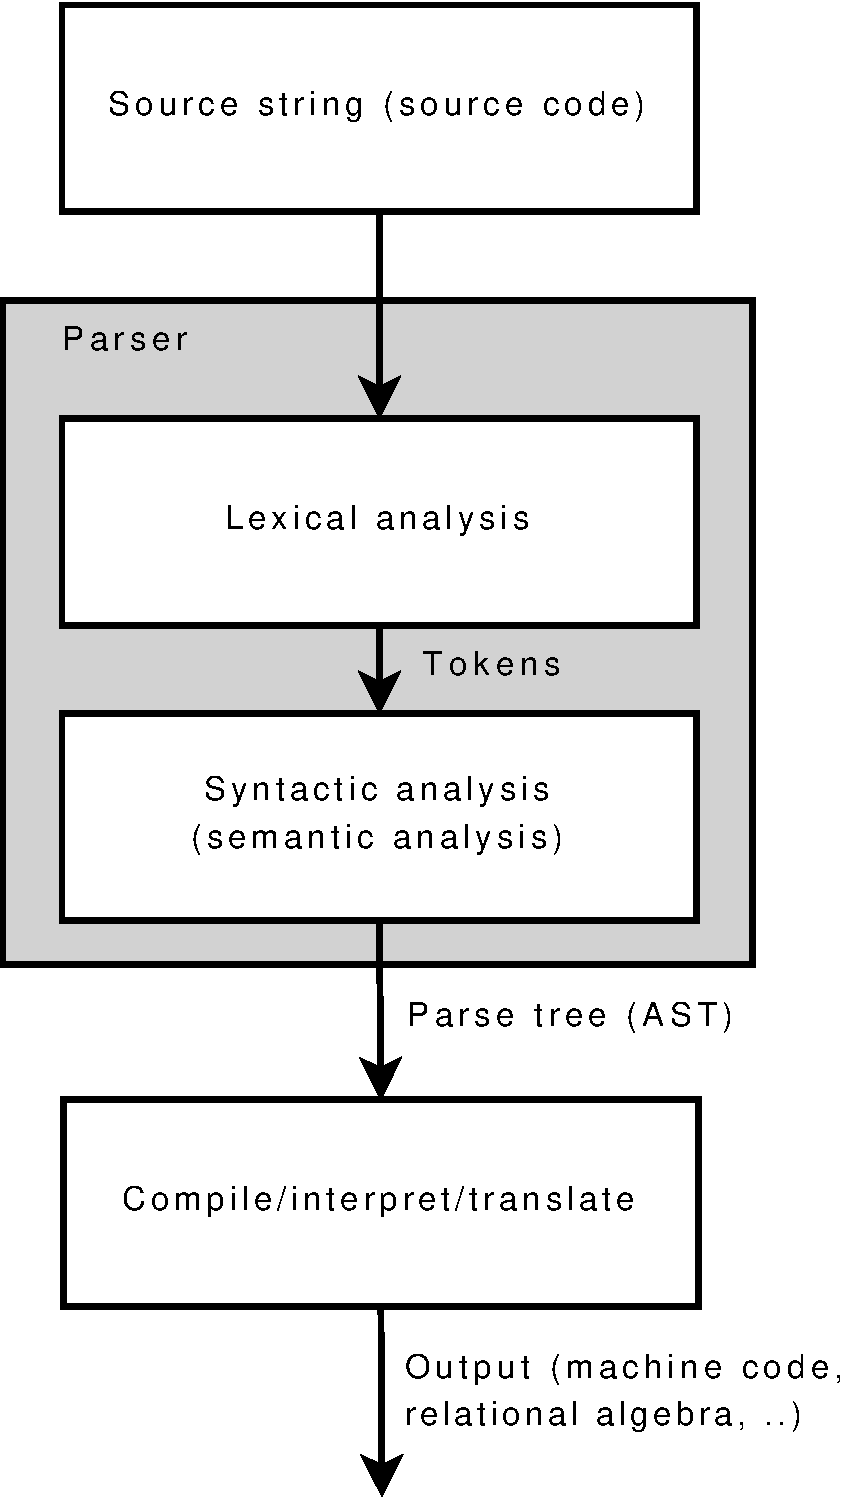
\includegraphics[scale=0.40]{diagrams/parser_overview}
  \caption{Typical compiler/interpreter data flow}
  \label{figure:parser:overview}
\end{figure}

\subsection{Common parser technologies}
There are two common types of parser technologies, \textit{top-down} and
\textit{bottom-up} parsers. As their names imply, these technologies differ in
the sense that top-down parsers will attempt to match production rules to the
input top-down, while bottom-up parsers will start at the ``bottom'' on the
terminal symbols and combine them into production rules. Often this is
implemented as a process of shift and reduce operations using stacks to hold
production rules and terminal symbols.

We refer to \cite{compiler_tech} for further in-depth information about parser
technologies, however it is important to note that typically a top-down parser
based on an LL\footnote{LL is a Left-to-right, Leftmost derivation
parser, using a top-down approach}-grammar with low token lookahead (typically
one token lookahead, aka LL(1)) will perform better and be subject to a high
number of optimizations, uot of which a few are described in
\cite{compiler_tech} and \cite{DBLP:books/cu/Appel1998c}.

\subsection{Parser generators}
Generelt om parser-generatorer
\subsubsection{Available implementations}
\subsubsection{ANTLR}

\subsection{AST construction and imaginary tokens}
Litt om hvordan AST'en blir konstruert i en LL-parser, og hvordan vi sproyter
inn imaginary tokens

\subsection{Tree parsing}
Tree parsing, henvise til metode eller flytte greiene fra metode og hit? Eller
noe.

\begin{itemize}
  \item Kort om forskjellige parser-teknologier
  \item Hvordan parseren vaar fungerer
  \item Hvordan ASTen ser ut\ldots kanskje nesten en egen subsection til
  dette.. iallefall i generelle trekk? hmmmmmz
  \item Syntax-tr\ae r og tre-parsing
  \item AST\_PATHEXPR\_SGL holder enkeltslash i begynnelsen av pathExprz
  \item Imagin\ae re tokens, og evt snakke om hvilke vi har lagt til i
  implementation?
\end{itemize}
